\chapter{Software}
Software pro Elektronickou hru Logic byl napsán v jazyce C++. Bylo využito skutečnosti, že mikrokontrolér ESP32-PICO podporuje Arduino 
framework. Pro psaní softwaru bylo použito vývojové prostředí Visual Studio Code. %kompilátor 

Pro programování inteligentních LED bylo využito již existující knihovny SmartLeds.h \cite{SmartLeds}.
Tato knihovna velmi usnadňuje softwarovou práci s těmito inteligentními LED. Obsahuje například funkci {\it show}, která umožní zobrazit 
nastavené barvy na všech inteligentních LED připojených k jednomu pinu mikrokontroléru ESP32-PICO. 

Celý software je rozdělen do dvou částí, počáteční inicializace a nekonečná smyčka programu. 

Po spuštění probíhá inicializace vstupně-výstupních pinů a teké inicializace proměnných. Všem inteligentním LED je vypnuto napájecí napětí. 
Dále je všem inteligentním LED nastavena barva na černou, tzn. LED nesvítí. Po kompletním nastavení se již čeká na stisk tlačítka "Nová hra". 

\section{Tlačítko Nová hra}
Když je stisknuto tlačítko "Nová hra", tak je všem inteligentním LED nastavena černá barva. Program načte stavy přepínačů. Pokud je nastavena hra pro 
jednoho hráče, tak je vygenerováno zadání. Pokud je hra s mezerou, tak je generace zadání rozšířena o černou barvu. Poslední přepínač určuje délku 
vygenerovaného zadání. V případě hry pro jednoho hráče je přepínač s mezerou ignorován. Následně je zapnuto napájecí napětí 
první části inteligentních LED a poté program přechází do druhé části, tj. nekonečné smyčky.

\begin{minipage}{\linewidth}
\begin{lstlisting}[frame=single,numbers=right,caption={Funkce pro vygenerování zadání.},label=lst:priklad.vypis.kodu.C,basicstyle=\ttfamily\small, keywordstyle=\color{black}\bfseries\underbar,]
void generate_task (Colors *task, int length, int diff){
    for(int i = 0; i < length; ++i)
        task[i] = Colors(esp_random() % (NUM_OF_COLORS - diff));
}     
void set_task(led_t &leds, Colors* array_task, int length){
    for (int i = 0; i < length; ++i){
        leds.pos = i;
        set_color(leds, array_task[i]); 
    } 
}   
\end{lstlisting}
\end{minipage} 

Nekonečná smyčka má dva hlavní úkoly. Detekuje stisknutí tlačítek a v pravidelných intervalech bliká kurzorem. Na konci každého průchodu smyčkou 
se obnoví zobrazení na inteligentních LED.

\section{Tlačítka interpretující šipky}
Po každém stisku některé z šipek program nejprve zjišťuje, zda je spuštěna hra pro jednoho, nebo pro dva hráče, a také, v případě hry pro dva
hráče, v jaké části inteligentních LED se právě nachází kurzor. Poté je kurzor dle dané šipky posunut buď o jedno pole vpravo, nebo o jedno 
pole vlevo, v rámci dané části inteligentních LED. 

Pokud se kurzor nachází na konci řádku a je stisknuto tlačítko "Šipka vpravo", je pozice přepočítána tak, aby se kurzor posunul na 
začátek téhož řádku. Pokud se kurzor nachází na začátku řádku a je stisknuto tlačítko "Šipka vlevo", je pozice přepočítána tak, aby se kurzor 
posunul na konec téhož řádku. 

\begin{minipage}{\linewidth}
\begin{lstlisting}[frame=single,numbers=right,caption={Funkce posouvající kurzor.},label=lst:priklad.vypis.kodu.C,basicstyle=\ttfamily\small, keywordstyle=\color{black}\bfseries\underbar,]
void shift_cursor (led_t &LED, Direct DIR, int length){
    if((DIR == RIGHT) && 
        !((LED.pos + 1 + LINE_LENGTH - length) % LINE_LENGTH))
        LED.pos -= LINE_LENGTH - (LINE_LENGTH - length) - 1;
    else if(DIR == RIGHT)
        LED.pos += 1;
    else if((DIR == LEFT) && 
            (LED.pos == 0 || !(LED.pos % LINE_LENGTH)))
        LED.pos += LINE_LENGTH - (LINE_LENGTH - length) - 1;
    else if(DIR == LEFT)
        LED.pos -= 1;
}   
\end{lstlisting}
\end{minipage} 
    
\section{Barevná tlačítka}
Po každém stisku barevného tlačítka program zjišťuje, zda je spuštěna hra pro jednoho, nebo pro dva hráče, a také, v případě hry pro dva hráče,
v jaké části inteligentních LED se právě nachází kurzor. Poté se nastaví v dané části daná barva LED na pozici kurzoru a kurzor se posune o 
jedno pole vpravo. Pokud se ve hře pro dva hráče nachází kurzor ve vyhodnocovací části, tak jsou stisky všech barev kromě červené a žluté 
ignorovány. Na konci průchodu smyčkou je tato změna zobrazena na inteligentních LED. 

\section{Tlačítko Potvrdit tah}
Po stisku tlačítka "Potvrdit tah"\  je zjištěno, zda je nastavena hra pro jednoho, nebo pro dva hráče. 

Pokud je nastavena hra pro jednoho hráče, tak dojde k vyhodnocení tahu a kurzor je posunut na první LED dalšího herního řádku. Pokud je již 
kurzor na posledním řádku, tak je zobrazeno zadání a kurzor přestává blikat. Pokud se shoduje herní kombinace se zadáním dříve, než na 
posledním řádku, tak je zobrazeno vyhodnocení i zadání. Kurzor přestává blikat a hra čeká na stisk tlačítka "Konec", nebo "Nová hra". 

Vyhodnocení probíhá ve dvou krocích. Nejdříve jsou hledány barvy na správných pozicích. Tyto barvy jsou ohodnoceny červeně. Pozice těchto 
barev jsou v dalších krocích vynechávány. Pokud je počet nalezených barev na shodných pozicích stejný, jako je délka zadání, tak vyhodnocení 
končí. Pokud tomu tak není, vyhodnocení pokračuje. Následně pokud je nalezena ve zbylých barvách barva, která je obsazena v zadání, tak je 
ohodnocena žlutou barvou. Každá ohodnocená barva se v dalších krocích již přeskakuje. 

Pokud je nastavena hra pro dva hráče, dojde k posunutí kurzoru na první LED části, která je právě na řadě. Pokud byl kurzor v zadání, posune
se do herního pole, pokud byl v herním poli, posune se do pole pro vyhodnocení a pokud byl kurzor v poli pro vyhodnocení, tak se přesune
do herního pole. 

Pokud má následující řádek vypnuto napájecí napětí, tak je toto napětí softwarově zapnuto. 

\section{Tlačítko Konec}
Pokud je stisknuto tlačítko "Konec", jsou všechny LED zhasnuty a poté je jim odpojeno napájecí napětí. Následně se čeká na stisk tlačítka
"Nová hra". 

\iffalse
\section{Funkce init}
Funkce {\it \_init\_} slouží pro inicializaci vstupně-výstupních pinů. Všechny piny, na kterých jsou připojena tlačítka, jsou nastaveny jako 
vstupní se zapnutým softwarovým pull-up rezistorem. Piny, na kterých jsou připojeny inteligentní LED, jsou nastaveny jako výstupní. Piny,
kterými je ovládáno připojení napájecího napětí jednotlivých částí inteligentních LED, jsou nastaveny jako výstupní a mají přednastavenou 
počáteční hodnotu. První část je zapnuta, zbylé 2 jsou vypnuty. Zbylým dvěma částem je napájení zapínáno až ve chvíli, kdy mají dané 
inteligentní LED svítit.

\begin{minipage}{\linewidth}
\begin{lstlisting}[frame=single,numbers=right,caption={Funkce pro úvodní inicializaci hardwaru.},label=lst:priklad.vypis.kodu.C,basicstyle=\ttfamily\small, keywordstyle=\color{black}\bfseries\underbar,]
void _init_ (){
    pinMode(LED_PIN_GAME, OUTPUT);
    pinMode(LED_PIN_TASK, OUTPUT);
    pinMode(LED_PIN_EVAL, OUTPUT);

    pinMode(SET_POWER_LEDS_1_TO_4, OUTPUT);
    pinMode(SET_POWER_LEDS_5_TO_7, OUTPUT);
    pinMode(SET_POWER_LEDS_8_TO_10, OUTPUT);

    pinMode(SW_ENTER, INPUT_PULLUP);
    pinMode(SW_RIGHT, INPUT_PULLUP);
    pinMode(SW_LEFT, INPUT_PULLUP);
    pinMode(SW_END, INPUT_PULLUP);
    pinMode(SW_NEW_GAME, INPUT_PULLUP);
    pinMode(SW_YELLOW, INPUT_PULLUP);
    pinMode(SW_ORANGE, INPUT_PULLUP);
    pinMode(SW_RED, INPUT_PULLUP);
    pinMode(SW_PURPLE, INPUT_PULLUP);
    pinMode(SW_BLUE, INPUT_PULLUP);
    pinMode(SW_GREEN, INPUT_PULLUP);

    digitalWrite(SET_POWER_LEDS_1_TO_4, POWER_ON); 
    digitalWrite(SET_POWER_LEDS_5_TO_7, POWER_OFF);
    digitalWrite(SET_POWER_LEDS_8_TO_10, POWER_OFF);
}
    \end{lstlisting}
    \end{minipage}

\section{Funkce ovládání tlačítek}
Zákmity tlačítek, které se dějí při stisku tlačítka, jsou řešeny hardwarových způsobem pomocí filtračních kondenzátorů. Proto tento probém
není řešen softwarově. Je ale možné, že hráč tlačítko drží po dobu delší, než trvá jeden programový cyklus. Došlo by tak k detekci více stisků.

Aby k této detekci nedocházelo, čeká se po detekci stisku na puštění tlačítka. Až poté je vykonáván příkaz. Tím je zaručeno, že se 
např. kurzor posune vždy jen o jedno pole. Pro zjednodušení tohoto zápisu byly vytvořeny funkce {\it is\_pressed(SW)} a {\it wait\_for\_btn\_release(SW)}.
Argumentem obou funkcí je pin tlačítka, na které se dotazuje/čeká. Funkce {\it is\_pressed} má návratovou hodnotu typu bool. Typ bool nabývá pouze 2 hodnot.
Těmito hodnotami jsou „true“\ = 1 (pravda) a „false“\ = 0 (nepravda). Pokud je tlačítko zmáčknuto, funkce vrátí „true“\, pokud tlačítko zmáčknuto není, 
funkce vrátí „false“\. Návratová hodnota je poté vyhodnocována v podmínce, zda je konkrétní tlačítko zmáčknuto. 

\begin{minipage}{\linewidth}
\begin{lstlisting}[frame=single,numbers=right,caption={Funkce pro detekci stisku tlačítka.},label=lst:priklad.vypis.kodu.C,basicstyle=\ttfamily\small, keywordstyle=\color{black}\bfseries\underbar,]
bool is_pressed(int btn){
    if(!digitalRead(btn))
        return true;
    return false;
}
\end{lstlisting}
\end{minipage}

\begin{minipage}{\linewidth}
\begin{lstlisting}[frame=single,numbers=right,caption={Funkce čekající na puštění tlačítka.},label=lst:priklad.vypis.kodu.C,basicstyle=\ttfamily\small, keywordstyle=\color{black}\bfseries\underbar,]
void wait_for_btn_release(int btn){
    while(!digitalRead(btn))
        delay(1);
}
\end{lstlisting}
\end{minipage} 

Tlačítka s barvami plní 2 funkce. Nejprve nastaví barvu dané LED a poté posunou kurzor o jedno pole vpravo. Tlačítka s šipkou posouvají kurzor daným směrem. 
Pro tyto 2 postupy vznikly funkce {\it set\_color(led, color)} a {\it shift\_cursor(led, direct, length)}.
Funkce {\it set\_color} má 2 argumenty. Jedním argumentem je barva LED, kterou má nastavit a druhým je řetězec LED, kde má tuto barvu nastavit.

\begin{minipage}{\linewidth}
\begin{lstlisting}[frame=single,numbers=right,caption={Ukázka funkce nastavující barvu inteligentním LED.},label=lst:priklad.vypis.kodu.C,basicstyle=\ttfamily\small, keywordstyle=\color{black}\bfseries\underbar,]
void set_color (led_t &LED, Colors COLOR){
    const int num_max = 32;
    switch (COLOR){
        case YELLOW:
        LED.leds[LED.pos] = Rgb{num_max, num_max, 0}; 
        break;
        case RED:
        LED.leds[LED.pos] = Rgb{num_max, 0, 0}; 
        break;
        case BLUE:
        ...
    } 
}    
\end{lstlisting}
\end{minipage} 

Funkce {\it shift\_cursor} posune kurzor vpravo, nebo vlevo, dle předaného argumentu. Pokud se kurzor nachází na konci herního řádku a je předán 
argument pro posun kurzoru vpravo, je pozice přepočítána tak, aby se kurzor posunul na začátek herního řádku. Pokud se kurzor nachází na začátku herního 
řádku a je předán argument pro posun kurzoru vlevo, je pozice přepočítána tak, aby se kurzor posunul na konec herního řádku. 

\begin{minipage}{\linewidth}
\begin{lstlisting}[frame=single,numbers=right,caption={Funkce posouvající kurzor.},label=lst:priklad.vypis.kodu.C,basicstyle=\ttfamily\small, keywordstyle=\color{black}\bfseries\underbar,]
void shift_cursor (led_t &LED, Direct DIR, int length){
    if((DIR == RIGHT) && 
      !((LED.pos + 1 + LINE_LENGTH - length) % LINE_LENGTH))
        LED.pos -= LINE_LENGTH - (LINE_LENGTH - length) - 1;
    else if(DIR == RIGHT)
        LED.pos += 1;
    else if((DIR == LEFT) && 
           (LED.pos == 0 || !(LED.pos % LINE_LENGTH)))
        LED.pos += LINE_LENGTH - (LINE_LENGTH - length) - 1;
    else if(DIR == LEFT)
        LED.pos -= 1;
}   
\end{lstlisting}
\end{minipage} 

\section{Zadání}
Vygenerování zadání a její následné uložení do inteligentních LED zajíšťují funkce {\it generate\_task(array, length, diff)} a {\it set\_task(leds, array, length)}.
Funkce generate task vygeneruje pomocí funkce {\it esp\_random} a matematické úpravy číslo od 0 do počtu barev. Každá barva je interpretována jiným číslem z tohoto 
rozsahu. Proměnná {\it diff} určuje, zda je může vygenerovat i černá (= mezera). Její hodnotu určuje stav přepínače. Proměnná {\it length určuje}, zda se vygeneruje zadání 
pro hru na 3 nebo 4 herní prvky. Její hodnota je také určována stavem přepínače. Zadání je uloženo do pole prvků, které je poté používáno pro vyhodnocení.

\begin{minipage}{\linewidth}
\begin{lstlisting}[frame=single,numbers=right,caption={Funkce pro vygenerování zadání.},label=lst:priklad.vypis.kodu.C,basicstyle=\ttfamily\small, keywordstyle=\color{black}\bfseries\underbar,]
void generate_task (Colors *task, int length, int diff){
    for(int i = 0; i < length; ++i)
        task[i] = Colors(esp_random() % (NUM_OF_COLORS - diff));
}      
\end{lstlisting}
\end{minipage} 

Funkce {\it set\_task} uloží hodnoty z pole, ve kterém je vygenerováno zadání, do inteligentních LED. Tam je uloženo a po zavolaní funkce {\it show} je ve správnou 
chvíli zobrazeno.

\begin{minipage}{\linewidth}
\begin{lstlisting}[frame=single,numbers=right,caption={Funkce pro vygenerování zadání.},label=lst:priklad.vypis.kodu.C,basicstyle=\ttfamily\small, keywordstyle=\color{black}\bfseries\underbar,]
void set_task(led_t &leds, Colors* array_task, int length){
    for (int i = 0; i < length; ++i){
        leds.pos = i;
        set_color(leds, array_task[i]); 
    } 
}      
\end{lstlisting}
\end{minipage}

\fi

\chapter{Způsob ovládání elektronické hry}
DPS obsahuje 3 přepínače SW13, SW14 a SW15. Těmito přepínači si hráč volí způsob hry.

Přepínač SW15 slouží k volbě hry pro jednoho, nebo pro dva hráče. Pokud hráč umístí přepínač do pozice ON, hra se přepne
do módu pro dva hráče. Rozdíl mezi těmito variantami hry je popsán v následujících kapitolách a funkce dalších přepínačů taktéž.

\section{Hra pro jednoho hráče}
Tato verze hry pro jednoho hráče má stejná pravidla jako desková hra Logic. Funkci druhého hráče nahrazuje řídicí elektronika
- mikrokontrolér ESP32-PICO.

Po zapnutí DPS stikne hráč tlačítko "Nová hra". V~této chvíli se vygeneruje zadání, které není vidět, a~první herní LED se 
rozbliká. Blikající herní LED značí pozici kurzoru. 
Kurzorem lze pohybovat pomocí šipek interpretovanými tlačítky "Šipka vpravo"\  a~"Šipka vlevo". Barvy herních LED se nastavují 
tlačítky ve spodní části DPS. Tato tlačítka jsou označena danými barvami. Pokud hráč zadá barvu, kterou zadat nechce, má dvě možnosti,
jak ji smazat. Kurzorem vybere danou barvu a buď ji hned změní na jinou barvu pomocí daného barevného tlačítka, nebo stiskne tlačítko 
stejné barvy a barva se smaže. 
Po zadání kombinace stiskne hráč tlačítko "Potvrdit tah". Po stisku tohoto tlačítka proběhne vyhodnocení a~to se zobrazí na 
vyhodnocovacích LED. 
Červená barva ve vyhodnocení značí, že hráč má v barevné kombinaci stejnou barvu se zadáním na stejné pozici. Žlutá barva znamená,
že hráč má v barevné kombinaci stejnou barvu se zadáním, ale na chybné pozici. Další barvy nejsou ohodnoceny. Pozice vyhodnocení
záměrně není shodná s pozicemi, kterých se hodnocení týká. Zleva jsou nejdříve umístěna všechna červená a až poté všechna žlutá 
hodnocení.

Po vyhodnocení se kurzor posune na první LED v~dalším řádku. Hra pokračuje obdobným způsobem.
Po zadání správné kombinace barev a~jejich pozic se rozsvítí zadání a~hra je u~konce. Pro novou hru stiskne hráč tlačítko
"Nová hra"\  a~pro ukončení tlačítko "Konec".
Po stisku tlačítka "Konec"\  zhasnou všechny herní, vyhodnocovací LED i~LED pro zadání. Poté je DPS připravena pro vypnutí
vypínačem.

Přepínač SW13 slouží pro nastavení, zda má zadání délku 3 nebo 4 pozice. Pokud hráč umístí přepínač do pozice ON, tak tím 
zvolí variantu hry na 4 pozice. V poloze 1 je zvolena varianta na 3 pozice a pohyb kurzoru se tím omezí pouze na první 3 pozice 
v řádku. Poslední pozice se ignoruje a také nikdy nesvítí.

Přepínač SW14 slouží pro nastavení, zda zadání může nebo nesmí obsahovat mezeru. Pokud dá hráč přepínač do pozice ON, 
tak v zadání mezera nikdy není. Pokud je v poloze 1, tak v zadání mezera být může. Není to ale nutností. 

\begin{figure}[!h]
    \begin{center}
        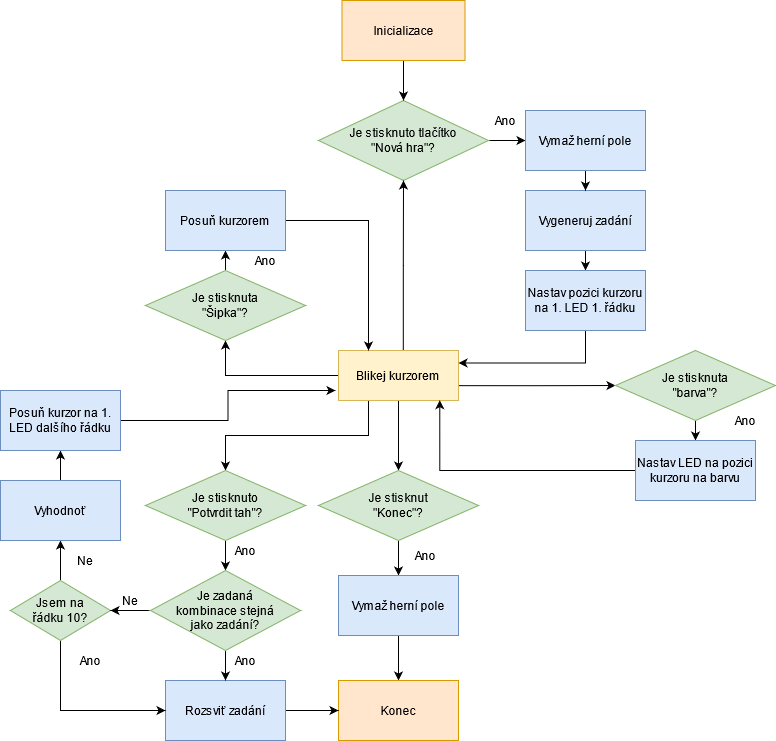
\includegraphics[scale=0.55]{obrazky/vyvojovy_diagram_1_hrac.png}
    \end{center}
    \caption[Vývojový diagram verze hry pro jednoho hráče]{Vývojový diagram verze hry pro jednoho hráče.}
    \end{figure}

\section{Hra pro dva hráče}
Varianta Elektronické hry Logic pro dva hráče má totožná pravidla s deskovou hrou. Po spuštění hry a stisku tlačítka "Nová hra"\ bliká 
kurzor v poli inteligentních LED se zadáním. První hráč zadává barvy pomocí barevných tlačítek a v poli LED se pohybuje pomocí šipek 
interpretovanými tlačítky. Hráč zadání zakryje stříškou a stiskne tlačítko „Potvrdit tah“. 

Po stisku zadání zůstane svítit a kurzor se přesune na první herní LED. Druhý hráč hledá zadanou kombinaci a tuto náhodnou kombinaci 
navolí pomocí barevných tlačítek. Kurzorem může taktéž pohybovat pomocí šipek interpretovanými tlačítky.
Pokud hráč zadá barvu, kterou zadat nechce, má dvě možnosti,
jak ji smazat. Kurzorem vybere danou barvu a buď ji hned změní na jinou barvu pomocí daného barevného tlačítka, nebo stiskne tlačítko 
stejné barvy a barva se smaže. Po zadání kombinace 
druhý hráč stiskne tlačítko „Potvrdit tah“\  a kurzor se přesune na první pozici vyhodnocovacího pole. 

První hráč má v tuto chvíli aktivní pouze šipky a červené a žluté barevné tlačítko. Červenou barvu zadává jako první a 
indikuje jí, že některá barva druhého hráče je obsažena v zadání, a to na totožné pozici. Poté zadává žlutou barvu, kterou 
udává, že některá z barev prvního hráče je obsažena v zadání, ale na jiné pozici, než kam ji druhý hráč umístil. Vyhodnocení 
hráč záměrně neumisťuje na pozice, kterých se hodnocení týká. Zpravidla se zleva umisťují nejdříve všechna červená a až poté 
všechna žlutá hodnocení. 

Po dokončení hodnocení první hráč stiskne tlačítko "Potvrdit tah"\  a kurzor se opět přesune na první pozici dalšího řádku herního pole. 
Hra dále pokračuje obdobným způsobem.
Pokud druhý hráč nalezne správnou kombinaci, pak první hráč odkryje zadání pro možnou kontrolu a hra je u konce. Pro možnost další 
hry stiskne jeden z hráčů tlačítko „Nová hra“. Celé herní, vyhodnocovací pole i pole se zadáním je smazáno a kurzor je znovu posunut 
na první pozici pole se zadáním. 

Přepínač SW13 slouží pro nastavení hry na 3 nebo 4 pole. Pokud hráči umístí přepínač do polohy ON, tak zvolí variantu hry na 4 pole. 
V poloze 1 zvolí variantu hry na 3 pole a omezí tím pohyb kurzoru pouze na 3 pole v každém řádku každé herní části. Poslední pozice
nikdy nesvítí a nikdy se také nehodnotí. 

Pozice přepínače SW14 se ve variantě hry pro dva hráče ignoruje. 

\begin{figure}[!h]
    \begin{center}
        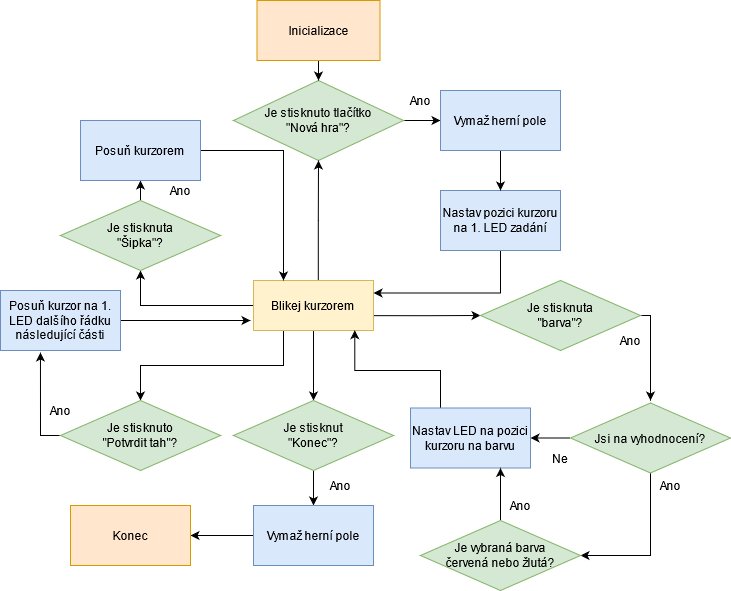
\includegraphics[scale=0.6]{obrazky/vyvojovy_diagram_2_hraci.png}
    \end{center}
    \caption[Vývojový diagram verze hry pro dva hráče]{Vývojový diagram verze hry pro dva hráče.}
    \end{figure}

\chapter{Krabička}
Krabička byla navržena v programu SolidWorks a vytištěna na 3D tiskárně. Spodní díl krabičky obsahuje 2 vyvýšené sloupky, ve kterých jsou otvory
na šrouby a matice. Vnitřní a nižší jsou určeny pro přišroubování DPS pomocí montážních otvorů a šroubů M3. Vnější otvory jsou poté pro přišroubování 
vrchního krytu krabičky. Otvor v horní části spodního dílu krabičky slouží pro umístění kolébkového vypínače. Na boční straně je také otvor
pro přivedení napájení USB konektorem.

Vrchní část krabičky obsahuje otvory pro LED a také pro tlačítka a přepínače. Tato část krabičky leží těsně nad DPS, aby nedocházelo k podsvitu LED přes
sebe a nemohlo tak docházet k podvodům během hry. 

Krabička také obsahuje tzv. stříšku, která je také součástí deskové hry. Tato stříška slouží pro zakrytí zadání ve hře pro dva hráče, kdy 
musí zadání svítit po celou dobu hry, aby byl druhý hráč schopen vyhodnocovat. Pro umístění stříšky slouží drážka ve vrchním dílu krabičky.

%obrázky

\chapter{Kompletace} 
Do spodního dílu krabičky byly do všech otvorů zalepeny matice M3 pomocí vteřinového lepidla. Do vrchního otvoru byl nasunut kolébkový vypínač, který
není třeba přilepit. Ke kolébkovému vypínači byly připájeny krátké drátové propojky.  

Do vnitřních otvorů byla přišroubována DPS pomocí šroubů M3$\times$6 se zápustnou hlavou. Klasické šrouby mají hlavičku, která je moc vysoká a krabička 
by nešla uzavřít. Zápustné šrouby jsou částečně zapuštěny do montážních otvorů DPS a tím je část hlavičky šroubu nad DPS nižší. 

Po uchycení DPS byly drátové prodlužky od kolébkového vypínače zasunuty do otvorů v DPS a připájeny.

Krabička byla následně přikryta vrchním dílem a přišroubována pomocí vnějších matic také šrouby M3$\times$6 se zápustnou hlavou. Ve vrchním dílu krabičky 
jsou otvory přizpůsobeny zápustným hlavám šroubů. Následně je možno zadání zakrýt stříškou, která se umisťuje do drážky ve vrchním dílu krabičky.
Po připojení jednoho z USB konektorů k napájecímu napětí je možno začít hrát.  
%obrázky